%& --translate-file=cp1250pl
%bez powyzszej linijki nie dzialaja polskie znaki (musi ona byc w pierwszej linii dokumentu
%%&platex --translate-file=il2-pl % przeyestowac z tym
\documentclass[a4paper,12pt]{article}
\usepackage[polish]{babel}
\usepackage[T1]{fontenc}
\usepackage[dvips]{graphicx}
%\usepackage{intendfirst}
\usepackage{times}
\usepackage{epsfig}
\usepackage{color}

%ustawienie wielkosci akapitu
%\setlength{\parindent}{0mm}
%%odst�p mi�dzy akapitami
%\setlength{\parskip}{2mm}

%ustawienia rozmiaru tekstu
    \textwidth 16cm
    \textheight 24cm 
    \topmargin -15mm
    \evensidemargin-3mm
    \oddsidemargin -3mm
    


\title{Salomon}

\author{Nikodem Jura \emph{(nico@icslab.agh.edu.pl)}
        \\
        Krzysztof Rajda \emph{(krzycho@student.uci.agh.edu.pl)}
        \\
        Jakub Ga�kowski \emph{(avi@student.uci.agh.edu.pl)}}               
        

\begin{document}

\maketitle
%wylaczenie numerowania na I stronie
\thispagestyle{empty}

\begin{center}
\textcolor{blue}{\underline{www.icslab.agh.edu.pl/$^{\sim}$nico/salomon}}
\end{center}

\begin{center}
Prowadz�cy: dr in�. Marek Kisiel-Dorohinicki
\end{center}

\newpage

%spis tresciz
\tableofcontents
\newpage

%reszta
\section{Wprowadzenie}

Salomon to system realizuj�cy koncepcj� \emph{Knowlege Mining}.
Sk�ada si� on z dw�ch zasadniczych cz�ci - pierwsz� z nich
stanowi silnik, kt�rego zadaniem jest zarz�dzanie i~uruchamianie
zada�. Druga cz�� to zbi�r wtyczek, dostarczaj�cych logik�
potrzebn� do skonfigurowania, wykonania i~wy�wietlenia rezultat�w
zadania. System jest otwarty - oznacza to, �e jego funkcjonalno��
mo�e by� w �atwy spos�b rozszerzalna poprzez dostarczenie nowych
wtyczek.

\begin{figure}[hbt]
	\centering
		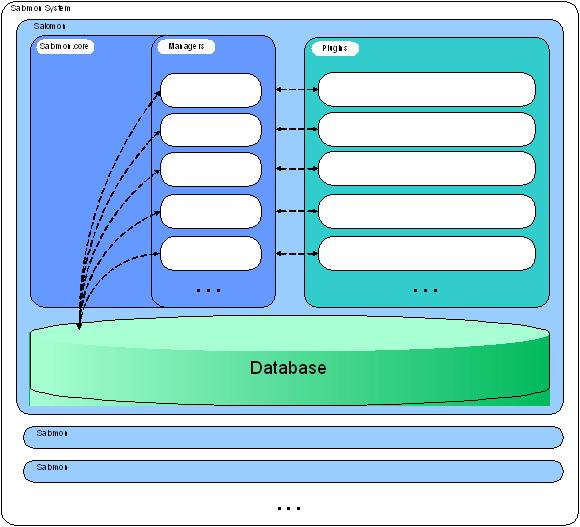
\includegraphics{arch}
	\caption{Architektura systemu}
	\label{fig:arch}
\end{figure}

\pagebreak
Podstawowe za�o�enia projektowe:
\begin{itemize}
    \item ca�a funkcjonalno�� w pluginach. J�dro systemu ma by� jak najmniejsze.
    Jego zadaniem jest stworzenie �rodowiska do realizacji logiki dostarczanej we wtyczkach
    \item otwarta~architektura. Wprowadzenie warstwy po�redniej pomi�dzy baz� danych~a wtyczkami.
    Jej zadaniem jest ukrycie sposobu organizacji danych przez
    wtyczkami. Otwarto��~architektury polega na mo�liwo�ci rozszerzenia tej warstwy
    \item niezale�no�� od platformy. System ma by� niezale�ny od platformy, mo�liwie �atwo przenaszalny.
    Poszczeg�lne cz�ci systemu mog� by� uruchamiane na r�nych
    platformach.
    \item �atwa~adaptacja funkcjonalno�ci zawartej w \emph{Vinlenie}.
    Projekt powsta� jako platforma uruchomieniowa dla logiki zaimplementowanej w programie \emph{Vinlen},
    stworzonego pod kierownictwem prof. Ryszarda Michalskiego.
\end{itemize}


Salomon ma na celu wyeliminowanie ogranicze� oryginalnego
\emph{Vinlena} poprzez wprowadzenie:

\begin{itemize}
    \item kolejkowania zada�
    \item rozproszenia
    \item r�wnoleg�o�ci
    \item rozszerzalno�ci (mechanizm wtyczek)
    \item przeno�no�ci (\emph{Java},\emph{Firebird})
\end{itemize}

\section{S�ownik}

\paragraph{Kontroler}
Kontroler to jedna instancja Salomona pracuj�ca w okre�lonym trybie: lokalnym, jako serwer lub klient. 

\paragraph{Menad�er} Klasy maj�ce w nazwie s�owo \emph{Manager} pe�ni� szczeg�ln� funkcj� - najcz�ciej odpowiadaj� za zarz�dzanie innymi klasami, z regu�y tymi, kt�re stanowi� reszt� nazwy (np. \emph{PluginManger} zarz�dza pluginami, \emph{ProjectManger} - projektami). G��wnym zadaniem menad�er�w jest odseparowanie wtyczek od operacji bezpo�rednio na danych.

\paragraph{Projekt}
W ramach projekt�w zapisywana jest konfiguracja systemu przed wykonaniem kolejki zada�. Zapisywana jest lista zada� do wykonania, ich ustawienia oraz pluginy, kt�re maj� by� u�yte do ich wykonania.

\paragraph{Plugin (wtyczka)}
Jest to zewn�trzny program odpowiedzialny za wykonanie konkretnego zadania. Nie jest integraln� cz�ci� systemu, w razie konieczno�ci jest pobierany z okre�lonej lokalizacji i przekazywane jest mu konkretne zadanie do wykonania.

\paragraph{�rodowisko}
Miejsce w kt�rym przechowywane s� zmienne �rodowiskowe.

\paragraph{Zmienna �rodowiskowa}
S�u�y do przekazywania informacji mi�dzy kolejnymi zadaniami.

\section{Architektura}

%diagram

System zosta� podzielony na 3 g��wne cz�ci: platform�, kontrolery
i~pluginy.

\subsection{Platforma}

Dostarcza podstawowej funkcjonalno�ci  umo�liwiaj�cej prac� ca�ego
systemu,  �aduje odpowiedni kontroler, wczytuje pluginy, uruchamia
zadania. Za poszczeg�lne zadania odpowiadaj� odpowiednie managery.
\\
Managery nie s� dost�pne bezpo�rednio z platformy, ale
przekazywane s� pluginom poprzez klas� \emph{DataEngine}. Dotyczy
to tylko klasy \emph{DataSetManager} i \emph{RuleSetManager},
pozosta�e nie s� dost�pne dla plugin�w. Plugin, zale�nie od
potrzeb, pobiera sobie z niego potrzebny mu manager i za jego
po�rednictwem wykonuje operacje na bazie danych.

\subsubsection{IManagerEngine}
Klasa zarz�dza pozosta�ymi managerami. Utrzymuje jedn� instancj� ka�dego z nich 
i udost�pnia je pozosta�ym klasom z platformy.

\subsubsection{DBManager}
Odpowiada za po��czenie z baz� danych. Dostarcza metod
zapewniaj�cych dost�p do danych przechowywanych w bazie. Swoj�
funkcjonalno�� udost�pnia odpowiednim managerom.

\subsubsection{DataSetManager}
Zarz�dza zbiorami danych. Pozwala tworzy� nowe podzbiory danych na
podstawie zawartych w bazie informacji oraz umo�liwia operowanie
na nich.

\subsubsection{RuleSetManager}
Zarz�dza regu�ami. Pozwala tworzy� nowe regu�y oraz
zarz�dza dost�pem do ju� istniej�cych.

\subsubsection{ProjectManager}
Zarz�dza projektami. Pozwala na utworzenie nowego
projektu, zapisanie bie��cego do bazy danych lub za�adowanie ju�
istniej�cego.

\subsection{Kontrolery}
Kontrolery odpowiadaj� za interakcj�
systemu z otoczeniem. W zale�no�ci od konfiguracji systemu przy
starcie uruchamiany jest jeden z kontroler�w. Kontrolery operuj�
na danych poprzez wsp�lny interfejs, a co za tym idzie: dane
utworzone poprzez jeden z nich s� dost�pne pomi�dzy kolejnymi
uruchomieniami programu dla pozosta�ych kontroler�w.

\subsubsection{LocalController}
 Jest najprostszym kontrolerem. Jego zadaniem jest
zarz�dzanie zadaniami wykonywanymi na lokalnym komputerze. S� one
wykonywane sekwencyjnie. Jego zadaniem jest dostarczenie
interfejsu u�ytkownika pozwalaj�cego na zarz�dzanie projektami,
pluginami i zadaniami.

\subsubsection{ServerController}
Zadaniem tego kontrolera jest dostarczenie interfejsu do
zarz�dzania zdalnymi kontrolerami (\emph{ClientController}). Po
uruchomieniu nas�uchuje na po��czenia od klient�w, rozdziela
zadania oraz wy�wietla ich wyniki.

\subsubsection{ClientController}
Zadaniem tego kontrolera jest odszukanie g��wnego kontrolera
(\emph{ServerController}), zarejestrowanie si� i udost�pnienia mu
swoich us�ug. Ta wersja kontrolera nie posiada GUI, zarz�dzanie
nim odbywa si� za pomoc� klasy \emph{ServerController}.


\subsection{Pluginy}
G��wna funkcjonalno�� zosta�a  przeniesiona
do plugin�w, zadaniem systemu jest tylko zarz�dzanie ich
wykonaniem. Dzi�ki takiemu podej�ciu system jest �atwo skalowalny
i rozszerzalny o nowe mo�liwo�ci. Ka�dy z plugin�w musi
implementowa� nast�puj�ce interfejsy:


\subsubsection{IGraphicPlugin}
Pozwala pobra� parametry od u�ytkownika, kt�re nast�pnie zostan�
przekazane do plugin�w  przed ich wykonaniem. Zawiera dwie metody:
\emph{getSettingsPanel()}  i \emph{getResultPanel()}.  Pierwsza z
metod zwraca panel s�u��cy do konfiguracji pluginu, druga � panel
na kt�rym prezentowane s� wyniki jego dzia�ania.

\subsubsection{IDataPlugin}

Posiada tylko jedn� metod� \emph{doJob()}. Przyjmuje ona jako
parametry obiekt klasy \emph{Environment}, reprezentuj�cy aktualny
stan systemu, \emph{DataEngine}, kt�ry umo�liwia operowanie na
bazie danych i \emph{ISettings}, reprezentuj�cy ustawienia
pluginu. Zwracany jest obiekt klasy \emph{IResult}, stanowi�cy
rezultat wykonania zadania.
\section{Opis bazy danych}sz

Do przechowywania danych wykorzystywanych przez system
wykorzystana zosta�a baza danych. Dane zosta�y zorganizowane w
nast�puj�cych tabelach:

\paragraph{Projects}

Tabela zawiera nag��wki projekt�w, do kt�rych odnosz� si� rekordy
z tabeli Tasks.

\begin{itemize}
    \item \emph{project\_id} - identyfikator projektu
    \item \emph{name} - nazwa
    \item \emph{info} - dodatkowy opis
\end{itemize}

\paragraph{Plugins}
Tabela zawiera informacje o pluginach, kt�re mog� by� wykorzystane
przez system. Przechowuje dane o ich nazwach i lokalizacjach, sk�d
mog� by� pobrane.
\begin{itemize}
    \item \emph{plugin\_id} - identyfikator pluginu
    \item \emph{name} - nazwa
    \item \emph{info} - dodatkowy opis
    \item \emph{location} - lokalizacja pluginu.
\end{itemize}

\paragraph{Tasks}
 Tabela zawiera zapis wykonania poszczeg�lnych task�w . Dla ka�dego
zadania przechowywane s� dane o pluginie, kt�ry zosta�
wykorzystany do wykonania zadania, projekcie, w ramach kt�rego
zadanie zosta�o zapisane, ustawienia, z jakimi zosta�o wykonane,
rezultat zadania oraz status, w jakim pozostaje po wykonaniu.

\begin{itemize}
    \item \emph{task\_id} - identyfikator taska
    \item \emph{project\_id} - identyfikator projektu, do kt�rego nale�y task
    \item \emph{plugin\_id} - identyfikator pluginu, kt�ry wykonywany jest w ramach tego taska
    \item \emph{name} - nazwa
    \item \emph{info} - dodatkowy opis
    \item \emph{plugin\_settings} - ustawienia pocz�tkowe pluginu
    \item \emph{plugin\_result} - rezultat dzia�ania pluginu
    \item \emph{status} - status wykonania taska
\end{itemize}

\paragraph{Datasets}
Zawiera nag��wki zbior�w zada�.
\begin{itemize}
    \item \emph{dataset\_id} - identyfikator zbioru danych
    \item \emph{dataset\_name} - nazwa
    \item \emph{info} - dodatkowy opis
\end{itemize}

\paragraph{Dataset\_items}
Zawiera definicje zbior�w zada�. Zbi�r danych definiowany jest
przez nazw� tabeli oraz warunki, jaki ograniczaj� rekordy w tej
tabeli.
\begin{itemize}
    \item \emph{dataset\_item\_id} - identyfikator elementu zbioru danych
    \item \emph{dataset\_id} - identyfikator zbioru danych do kt�rego nale�y
element
    \item \emph{table\_name} - nazwa tabeli
    \item \emph{condition} - warunek ograniczaj�cy zakres danych
\end{itemize}
    Relacje mi�dzy nimi zobrazowane s� na
poni�szym rysunku:

\section{Tworzenie w�asnego pluginu}

	System, dzi�ki swej elastycznej architekturze, pozwala u�ytkownikowi na rozszerzanie jego mo�liwo�ci poprzez definiowanie przez niego w�asnych plugin�w. Ca�a funkcjonalno�� zwi�zana z przetwarzaniem plugin�w, konfigurowaniem ich, prezentacj� wynik�w ich dzia�ania oraz komunikacj� przez sie� ukryta jest przed tw�rc� pluginu i nie musi by� brana pod uwag� przy jego projektowaniu i implementacji. Jedyne co musi on zrobi� to zaimplementowa� opisane poni�ej interfejsy.
By system m�g� skorzysta� z nowych plugin�w nale�y doda� go do systemu, umo�liwiaj�c mu tym samym zlokalizowanie i �ci�gni�cie pluginu. 

Obecna wersja systemu obs�uguje tylko pluginy w postaci archiw�w jar.

Poni�ej zamieszczony jest schemat przyk�adowego pluginu:

\begin{figure}[!hb]
	\centering
		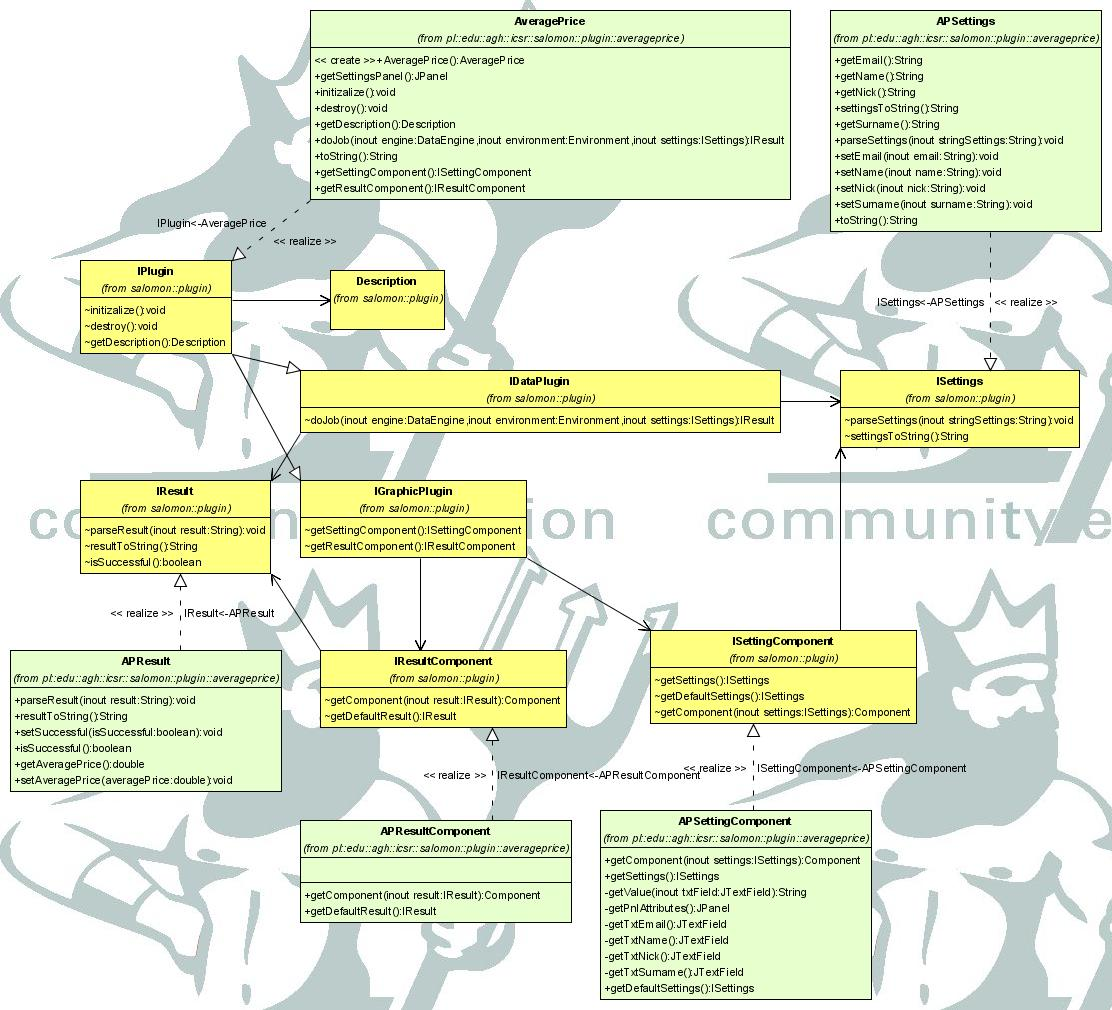
\includegraphics[scale=0.40]{img/average_price_plugin}
	\caption{Przyk�adowy plugin}
	\label{fig:AveragePricePlugin}
\end{figure}

Klasy zaznaczone na zielono i rozpoczynaj�ce si� od liter \emph{AP} to przyk�adowe implementacje interfejs�w plugni�w (kolor ��ty).  

	\subsection{Interfejsy plugin�w}

Ka�dy plugin by m�g� by� przetwarzany przez system musi
implementowa� nast�puj�ce \mbox{interfejsy:}

\subsubsection{IPlugin}

    \paragraph{getDescription()} - zwraca obiekt klasy
    \emph{Description} zawieraj�cy opis pluginu (nazw�, lokalizacj�,
    wersj� itp.)

\subsubsection{IDataPlugin}
    \paragraph{doJob()} - metoda wykonuje g��wne zadanie pluginu

\subsubsection{IGraphicPlugin}

    \paragraph{getSettingComponent()} - zwraca obiekt
    implementuj�cy interfejs \emph{ISettingComponent}

    \paragraph{getResultComponent()} - zwraca obiekt implementuj�cy
    interfejs \emph{IResultComponent}\\



Interfejs \emph{IGraphicComponent} zapewnia interakcj� z
u�ytkownikiem. Jego metody zwracaj� komponenty pozwalaj�ce na
modyfikacj� ustawie� pluginu oraz na wy�wietlenie rezultatu jego
dzia�ania. Obiekty zwracane przez metody tego interfejsu
implementuj� interfejsy:

	\subsubsection{ISettingComponent}

    \paragraph{getComponent(ISettings settings)} - zwraca graficzny
    komponent s�u��cy do edycji ustawie� pluginu. Jest on wype�niany
    warto�ciami przekazanymi w obiekcie \emph{ISettings}.

    \paragraph{getSettings()} - zwraca ustawienia pluginu

    \paragraph{getDefaultSettings()} - zwraca domy�lne ustawienia
    pluginu. Wykorzystywana gdy u�ytkownik nie wprowadzi� w�asnych
    ustawie�

	\subsubsection{IResultComponent}

    \paragraph{getComponent(IResult result)} - zwraca graficzny
    komponent wy�wietlaj�cy rezultat wykonania pluginu. Wype�niany
    jest on na podstawie obiektu  \emph{IResult} zwr�conego wcze�niej
    przez metod� \emph{doJob()}.

    \paragraph{getDefaultResult()} - zwraca domy�lny rezultat wykonania pluginu

	\subsubsection{ISettings}Implementowany przez obiekt reprezentuj�cy
	ustawienia pluginu.

    \paragraph{parseSettings(String settings)} - metoda inicjalizuje obiekt klasy
    \emph{ISettings}  na podstawie jego  tekstowej reprezentacji.
    U�ywana przy �adowaniu ustawie� pluginu z  bazy danych

    \paragraph{settingsToString()} - zwraca tekstow� reprezentacj�
    obiektu klasy \emph{ISettings}. U�ywana przy zapisie ustawie� pluginu do
    bazy danych

	\subsubsection{IResult} Implementowany przez obiekt reprezentuj�cy rezultat
	dzia�ania pluginu.

    \paragraph{parseResult(String result)}- metoda inicjalizuje obiekt klasy
    \emph{IResult}  na podstawie jego  tekstowej reprezentacji.
    U�ywana przy �adowaniu rezultatu dzia�ania pluginu z bazy danych

    \paragraph{resultToString()} - zwraca tekstow� reprezentacj� obiektu klasy
    \emph{IResult}. U�ywana przy zapisie rezultatu dzia�ania pluginu do bazy danych

\section{Uruchomienie}
Do uruchomienia programu konieczne jest zainstalowanie w systemie \emph{Java Runtime Environment} , w wersji 1.5. Je�li program ma dzia�a� z wykorzystaniem niezale�nego serwera bazy danych \emph{Firebird}, to nale�y zainstalowa� dodatkowo baz� \emph{Firebird}.

Program mo�e dzia�a� w 3 trybach (jako serwer, klient lub lokalnie) i na dwa sposoby ��czy� si� z baz� danych (poprzez serwer lub bez niego), zale�nie od wpis�w w pliku konfiguracyjnym. 
Aby uruchomi� go w odpowiedniej konfiguracji, nale�y rozpakowa� go i zmodyfikowa� domy�lne ustawienia pliku konfiguracyjnego. Program dostarczany jest z przyk�adow� baz� danych w kt�rej zdefiniowane s� odpowiednie tabele i lokalizacje plugin�w oraz z przyk�adowymi pluginami. 
Dla u�ytkownik�w, kt�rzy chc� stworzy� w�asn� baz� danych w katalogu db umieszczony zosta� skrypt, tworz�cy tabele niezb�dne do pracy programu i uruchomienia dostarczonych plugin�w (crebas.sql).

\subsection{Plik konfiguracyjny}
G��wnym plikiem konfiguracyjnym programu jest config.properties.
Zawiera on nast�puj�ce klucze:

\begin{itemize}
\item \emph{HOSTNAME} - identyfikator sieciowy komputera, na kt�rym zainstalowana jest baza danych. Uwzgl�dniany jest tylko w przypadku, gdy program ��czy si� z baz� danych przy u�yciu serwera Firebird.

\item \emph{DB\_PATH} - lokalizacja bazy danych. Gdy program dzia�a z serwerem Firebird jest to lokalizacja bezwzgl�dna, w przeciwnym przypadku - wzgl�dem katalogu instalacyjnego.

\item \emph{USER} - nazwa u�ytkownika, kt�ry loguje si� do bazy

\item \emph{PASSWD} - has�o u�ytkownika

\item \emph{EMBEDDED} - okre�la, spos�b po��czenia z baz� danych
\subitem \emph{N} - z wykorzystaniem serwera
\subitem \emph{Y} - przy u�yciu dll-a

\item \emph{SERVER\_HOST} - nazwa komputera, na kt�rym zainstalowany jest Salomon w wersji server

\item \emph{SERVER\_PORT} - port na kt�rym nas�uchuje server

\item \emph{MODE - tryb} uruchomienia
\subitem \emph{local} - lokalnie
\subitem \emph{client} - klient
\subitem \emph{server} - serwer

\end{itemize}

Pozosta�e warto�ci nie powinny by� modyfikowane przez u�ytkownika.

\subsection{Ustawienia pliku konfiguracyjnego}
\paragraph{Tryb serwera}
\begin{itemize}
    \item \emph{MODE=server}
    \item \emph{SERVER\_HOST=IP hosta}
    \item \emph{SERVER\_PORT=nr portu}
\end{itemize}

\paragraph{Tryb klienta}
\begin{itemize}
    \item \emph{MODE=server}
    \item \emph{SERVER\_HOST=IP sewera}
    \item \emph{SERVER\_PORT=nr portu na kt�rym nas�uchuje serwer}
\end{itemize}

\paragraph{Tryb lokalny}
\begin{itemize}
    \item \emph{MODE=local}
\end{itemize}

We wszystkich trybach mo�liwe jest ustawienie po��czenie z baz� danych za pomoc� serwera Firebird lub przy u�yciu dll-a (klucz \emph{EMBEDDED}).

\section{Interfejs u�ytkownika}

\subsection{Tryb serwera}
G��wnym zadaniem systemu jest umo�liwienie definiowania i wykonywania zada� w oparciu o dost�pne pluginy. Gdy program dzia�a w trybie serwera po lewej stronie widoczna jest lista pod��czonych klient�w. Wszystkie opisane poni�ej operacje wykonywane s� dla aktualnie wybranego klienta.

\subsubsection{Zadania}
Aby zdefiniowa� nowe zadanie, nale�y wybra� plugin, za pomoc� kt�rego b�dzie ono realizowane oraz skonfigurowa� jego ustawienia. Plugin nale�y wybra� z listy dost�pnych plugin�w, znajduj�cej si� na �rodku g��wnego okna programu. Po wybraniu pluginu i naci�ni�ciu przycisku ze strza�k� w prawo znajduj�cego si� miedzy panelem z pluginami a panelem z zadaniami pojawia si� okienko, w kt�rym nale�y wprowadzi� nazw� zadania. 


%\paragraph{@@@PIPCZER}
\paragraph{}

Po potwierdzeniu nazwy zostanie utworzone nowe zadanie i dodane do listy zada�. Ka�de z zada� mo�na skonfigurowa� przed wykonaniem, w tym celu nale�y nad wybranym zadaniem wywo�a� menu kontekstowe (prawym klawiszem myszy) i wybra� opcj� \textbf{Settings}. Po jej wybraniu pojawi si� okienko s�u��ce do konfiguracji zadania - mo�e by� r�ne, zale�nie od pluginu kt�ry ma by� wykonany w ramach zadania. 

%\paragraph{@@@PIPCZER}


\paragraph{}
Po skonfigurowaniu zada� nale�y zatwierdzi� list� zada� do wykonania za pomoc� klawisza \textbf{Apply}. Je�li zadania nie zosta�y wcze�niej zapisane w ramach projektu, pojawi si� okienko w kt�rym nale�y poda� nazw� projektu. Po poprawnym zapisaniu projektu mo�na wykona� zaplanowane zadania. Zostan� one wykonane  w takiej kolejno�ci, w jakiej znajduj� si� one na li�cie zada�. Mo�liwa jest zmiana tej kolejno�ci - s�u�� do tego przyciski ze strza�kami znajduj�ce si� po prawej stronie panelu z zadaniami. Je�li zostanie ustalona ostateczna kolejno�� zada�, mo�na je wykona� za pomoc� przycisku Run.

\paragraph{}
Po wykonaniu zada� mo�na obejrze� ich rezultaty. W tym celu nale�y z menu kontekstowego dla zada� wybra� opcj� \textbf{Result}. Po jej wybraniu pojawi si� okienko prezentuj�ce wyniki wykonania danego zadania. Jego wygl�d, podobnie jak w przypadku ustawie� zada�, zale�y od pluginu.

\subsubsection{Pluginy}
Lista plugin�w tworzona jest na podstawie odpowiednich wpis�w w bazie danych. Mo�na j� jednak  modyfikowa� - dodawa�, usuwa� lub modyfikowa� dane pluginy. S�u�� do tego odpowiednie opcje z menu kontekstowego wywo�ywanego dla plugin�w. 

%\paragraph{@@@PIPCZER}


\subsubsection{Projekty}

Konfiguracja plugin�w oraz lista zada� zapisywana jest w ramach projekt�w. Dzi�ki temu mo�na zdefiniowa� r�ne listy zada� i wykonywa� je wielokrotnie, bez potrzeby ich ponownego tworzenia i konfiguracji. Aby za��dowa� istniej�cy projekt nale�y z menu g��wnego wybra� pozycj� \textbf{Projects$\rightarrow$Open Project}. Spowoduje to wy�wietlenie listy zapisanych projekt�w i umo�liwi wyb�r projektu do za�adowania. 

\subsection{Tryb klienta}
Program pracuj�cy w tym trybie nie posiada interfejsu u�ytkownika, jego konfiguracja odbywa si� z serwera.

\subsection{Tryb lokalny}
Interfejs dla programu dzia�aj�cego w trybie lokalnym zbli�ony jest do programu w trybie serwera. Nie posiada on jednak listy pod��czonych klient�w, gdy� sam wykonuje zdefiniowane zadania, czyli zachowuje si� jak po��czenie dw�ch program�w dzia�aj�cych w trybie serwera i klienta.

\subsection{SQL Console}
W trybie serwera oraz w trybie lokalnym z menu Tools dost�pny jest program SQL Console. Pozwala on na wykonywanie zapyta� SQL-owych, przez co umo�liwia administracj� projektami, pluginami i zadaniami oraz innymi tabelami wykorzystywanymi przez system.


\section{Rozproszenie i r�wnoleg�o��}
\paragraph{}
G��wnymi celami przy projektowaniu cz�ci systemu odpowiedzialnych za rozproszenie systemu by�a �atwo�� wymiany architektury, na kt�rej zosta�o oparte rozproszenie. W naszym przypadku zosta�o zastosowane RMI. System zosta� napisany w Javie i nie zale�a�o nam przeno�no�ci kodu pomi�dzy r�ne platformy programistyczne. Samo j�dro systemu ma by� szybkie, liniowe i sekwencyjne, bez mo�liwo�ci wykonywania r�wnoleg�ych zada�, a r�wnoleg�o�� wykonywana jest na poziomie kontroler�w. 


\paragraph{Stworzyli�my dwa kontrolery:}

\begin{itemize}
\item \emph{ServerController} - jego zadanie jest nas�uchiwanie na po��czenia klient�w, udost�pniaj�cych swoje mo�liwo�ci. Rozdziela on zadania pomi�dzy r�nych klient�w i zbiera od nich wyniki.

\item \emph{ClientContoller} - zadanie tego kontrolera jest zainicjalizowanie j�dra systemu, zarejestrowanie si� u ServerContollera i odbieranie i wykonywanie zada� otrzymanych od serwera i wysy�anie mu wynik�w. Kontroler ten nie posiada GUI, jego konfiguracja odbywa si� poprzez odpowiednie wpisy w pliki konfiguracyjne.
\end{itemize}

\paragraph{}
Aby mo�liwe by�o wykonanie zadania na kliencie, serwer i klient musz� posiada� w�asn� instancj� plugin�w. Za�o�enie to podyktowane jest tym, �e serwer wykorzystuje plugin do utworzenia danych wej�ciowych dla zadania oraz do prezentacji wynik�w, a klient wykorzystuje plugin do odpalenia zadania. Dzi�ki takiemu podej�ciu minimalizowany jest ruch pomi�dzy poszczeg�lnymi elementami systemu. Gdy serwer chce zleci� klientowi zadanie wysy�a mu adres, z kt�rego klient mo�e pobra� dany plugin (aktualnie to FTP, HTTP). Klient sprawdza wersje pluginu na podstawie podanej lokalizacji, w razie posiadania starszej wersji lub jego braku, klient przed wykonaniem zadania pobiera plugin do swego lokalnego cache'a. 


\subsection{Struktura klas}
Struktura klas, kt�re uczestnicz� w komunikacji jest zarazem warstwowa i drzewiasta. 

\subsubsection{Drzewiasta} 
Ze wzgl�du na funkcjonalno�� mo�na wyr�ni� drzewiast� struktur� klas, implementuj� podany interfejsy. Na szczycie drzewa znajduje si� IManagerEngine. Interfejs ten s�u�y do zarz�dzania poszczeg�lnymi menad�erami.
 
\paragraph{Pluginy}
\begin{itemize}
\item \emph{IPluginManager} -  s�u�y do zarz�dzania pluginami
\item \emph{IPlugin} -  udost�pnia funkcjonalno�� plugin�w
\end{itemize}

\paragraph{Zadania}
\begin{itemize}
\item \emph{ITaskManager} - s�u�y do zarz�dzania zadniami
\item \emph{ITask} - reprezentuje zadanie w systemie
\item \emph{ISettings} - reprezentuje ustawienia dla zadania 
\item \emph{IResult} - reprezentuje wynik zadania
\end{itemize}

\paragraph{Projekty}
\begin{itemize} 
\item \emph{IProjectManager} - s�u�y do zarz�dzania projektami
\item \emph{IProject} - reprezentuje projekt w systemie
\end{itemize}

\subsubsection{Warstwowa} 

\paragraph{Wyr�niamy trzy warstwy:}

\paragraph{}
W sk�ad pierwszej warstwy wchodz� nast�puj�ce klasy: \emph{ManagerEngine, PluginManager, Plugin, TaskManager, Task, ProjectManager, Project}. Warstwa ta wyst�puje w wersji rozproszonej i�nierozproszonej. W tej warstwie zawarta jest g��wna logika systemu. 

\paragraph{}
Druga warstwa to warstwa odpowiedzialna za komunikacj� po stronie klienta. W sk�ad warstwy tej wchodz� interfejsy: \emph{IRemoteManagerEngine, IRemotePluginManager, IRemotePlugin, IRemoteTaskManager, IRemoteTask, IRemoteProjectManager, IRemoteProject} oraz odpowiednio klasy implementuj�ce interfejsy:  \emph{RemoteManagerEngine, RemotePluginManager, RemotePlugin, RemoteTaskManager, RemoteTask, RemoteProjectManager, RemoteProject}. Interfejsy wchodz�ce w sk�ad tej warstwy s� to w wi�kszo�ci przypadk�w dok�adne odpowiedniki interfejs�w, ale bez fragmentu �Remote�. Interfejsy te s� zdalne.

\paragraph{}
Trzecia warstwa to warstwa odpowiedzialna za ukrycie po stronie serwera faktu zdalno�ci obiekt�w.  W sk�ad warstwy tej wchodz�: \emph{ManagerEngineProxy, PluginManagerProxy, PluginProxy, TaskManagerProxy, TaskProxy, ProjectManagerProxy, ProjectProxy}. Klasy te to proste wrappery na zdalne obiekty, kt�re implementuj� odpowiednie interfejsy z j�dra systemu. Deleguj� wywo�ania metod do zdalnych obiekt�w i zajmuj� si� obs�ug� zdalnych wyj�tk�w. 

\paragraph{}
Dzi�ki zastosowaniu budowy warstwowej interfejsy z j�dra systemu nie musza dziedziczy� po Remote ani wyj�tk�w \emph{RemoteException}, a podmiana technologii s�u��cej do komunikacji, to tylko wymiana drugiej i trzeciej warstwy, bez ingerencji w logik� systemu. Nie ma wymagania na to, aby zdalne interfejsy dok�adnie odpowiada�y swoim odpowiednikom z j�dra.

\paragraph{}
Dodatkowo na potrzeby GUI serwera zosta�a stworzona kolejna warstwa, w kt�rej sk�ad wchodz�: \emph{ManagerEngineHolder, PluginManagerHolder, ProjectManagerHolder, TaskManagerHolder}. Zadaniem tej warstwy jest zapewnienie bezpiecze�stwa zmiany obecnie konfigurowanego klienta. Klasy te to wrappery, kt�re przechowuj� instancje odpowiednich klas z warstwy trzeciej. Dzi�ki takim wrapperom podmiana aktualnie konfigurowanego klienta nast�puje tylko w jednym miejscu. Podmiana polega na podmianie instancji przechowywanych w Holderach. Warstwa zabezpiecza przed sytuacj�, w kt�rej nie wszystkie instancje w GUI wskazuj� na jednego klienta. 

Warstwowa struktura klas

\begin{figure}[htb]
	\centering
		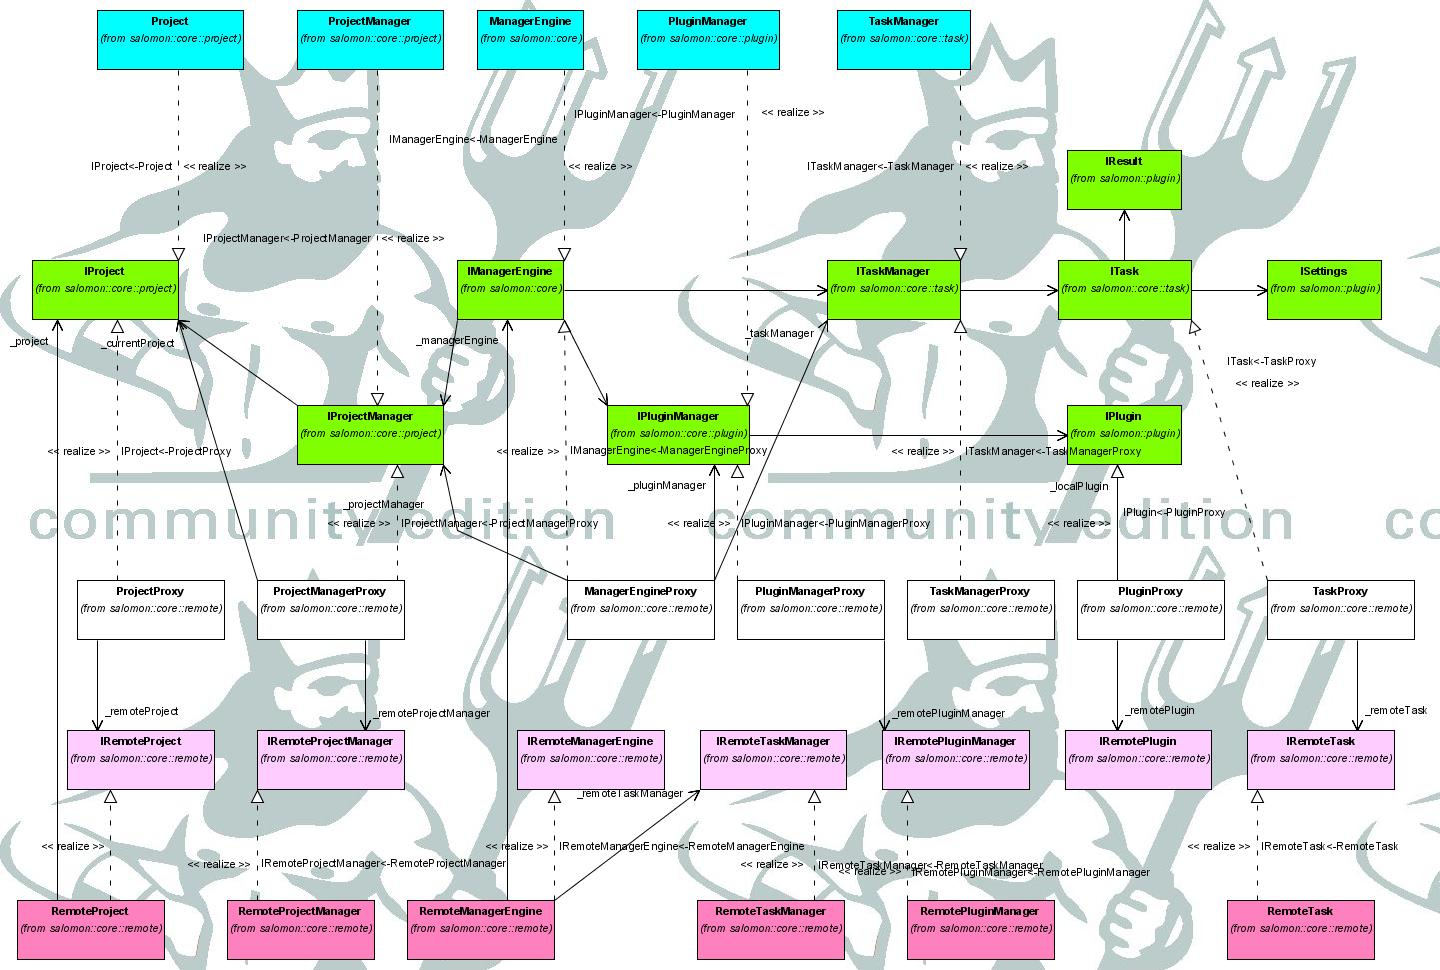
\includegraphics[scale=0.45, angle=270]{Communication.jpg}
	\caption{Warstwowa struktura klas}
	\label{fig:Communication}
\end{figure}

\section{Za�o�enie implementacyjne}
W czasie produkcji systemu stosowali�my nast�puj�ce zasady:

\subsection{Kontrola wersji}
Ca�y kod oraz inne zasoby wykorzystywane w programie znajduj� si� pod kontrol� wersji. U�ywany do tego jest  \emph{Subversion} (nast�pca CVS-a) i odpowiednie pluginy zapewniaj�ce jego integracj� z edytorem oraz systemem operacyjnym. Zapewnia to pe�n� synchronizacj� kodu na wszystkich komputerach, na kt�rych mo�e on by� modyfikowany.

\subsection{Wsp�lny edytor}
U�ywany jest wsp�lny edytor - \emph{Eclipse}. Dzi�ki mo�liwo�ci eksportowania ustawie� u�ywane jest  identyczne formatowanie kodu, co pomaga utrzyma� przejrzysto�� i czytelno�� kodu. 

\subsection{Testowanie jednostkowe} 
W celu testowania funkcjonalno�ci wykorzystujemy mechanizm \emph{JUnit}. 

\subsection{GUI testowanie}
W celu weryfikowania poprawno�ci interfejsu u�ytkownika stworzone zosta�y skrypty dla programu Abbot. Jego zadaniem jest odtworzenie nagranych sekwencji wykonywanych  przez  u�ytkownika w czasie obs�ugi programu. W po��czeniu z runtime-ow� weryfikacj� kontrakt�w stanowi to silny mechanizm weryfikacji jako�ci produktu

\subsection{Kontrakty}
W kodzie zosta�y wprowadzone mechanizmy zaczerpni�te z j�zyka  \emph{Eiffel} - tzw. kontrakty. Polega to na tym, �e w komentarzach dla klas oraz metod zawarte s� warunki, sprawdzaj�ce poprawno�� stanu, w jakim znajduje si� system. Kontrakty stanowi� dodatkow� informacj� dla programisty wykorzystuj�cego dan� klas� lub interfejs. Dodatkowo wykorzystywany jest kompilator, kt�ry kompiluje tak�e kod kontrakt�w i w razie ich z�amania rzuca wyj�tki.

\subsection{Automatyczne budowanie projektu} 
W celu zautomatyzowania procesu budowania projektu wykorzystany zosta� program  \emph{Ant}. Automatyzuje on proces tworzenia projektu od kompilacji, a� do wygenerowania instalatora.

\subsection{Instalator}
By upro�ci� proces instalacji dla u�ytkownika ko�cowego utworzone zosta�y skrypty tworz�ce instalator. Jako program do utworzenia instalatora wykorzystywany jest program  \emph{IzPack}.

\subsection{Mechanizmy lokalizacyjne}
Wszystkie teksty u�yte w interfejsie u�ytkownika pobierane s� z odpowiednich plik�w, co pozwala na �atw� lokalizacj� programu

\subsection{Konfiguracja}
Konfiguracja programu wczytywana jest z odpowiednich plik�w konfiguracyjnych. Pozwala to na �atw� zmian� zachowania programu (np. zmian� kontrolera). 

\subsection{Logowanie}
Do �ledzenia przebiegu wykonania programu wykorzystywany jest log4j. Wprowadza on elastyczny model logowania. 

\subsection{Zarz�dzanie projektem}
Jak system zarz�dzania projektem wybrali�my Gemini - system wspomagania pracy grupowej oparty na ASP.NET. System wspomaga wszelkie dziedziny �ycia projektu, poczynaj�c od przydzia�u zada� dla poszczeg�lnych developer�w, kontroli stanu ich wykonania, estymacji czasu pracy nad danym zagadnieniem, po zarz�dzanie projektem jak ca�o�ci� czyli wyznaczanie milestone'�w oraz przypisywania do nich zada�, generacja diagram�w Gantta, zarz�dzanie zasobami ludzkimi itp. 

%\subsection{CMS}
%Jako CMS(Content Management System) dla naszej strony zosta� u�yty projekt Mambo 4.9.1a. Jest to bardzo wygodny i %elastyczny w u�ytkowaniu system kontroli tre�ci. System ma budow� modu�ow� dzi�ki czemu mo�emy w ka�dej chwili rozszerzy� %jego funkcjonalo��. Opr�cz standardowych modu��w jakie dostarczane s� z dystrybucj� Mambo do��czyli�my Forum dyskusyjne %(SimpleBoard) oraz galeri� (RSGallery). Dodatkow� mo�liwo�ci� jest wrappowanie innych projekt�w dzi�ki czemu uda�o nam %sie bez wi�kszych problem�w doda� modu�y bezpo�rednio nie wspierane przez Mambo, jak Bugzilla czy Wiki.


%\subsection{Maven}
%W projekcie u�yli�my r�wnie� mavena. Jest to bardzo u�yteczne narz�dzie do zarz�dzania buildami, jak r�wnie� tworzeniem raport�w na temat posuwaj�cych si� prac. Aktualnie podpi�li�my nast�puj�ce raporty:
%\begin{itemize}
%	\item Changes\\
%	w estetyczny spos�b pokazuje wersje, i zmiany jakie w nich zasz�y
%	\item Checkstyle\\
%	raport z checkstyle'a \href{http://checkstyle.sourceforge.net/}{http://checkstyle.sourceforge.net/}, najpopularniejszego chyba darmowego narz�dzia do statycznej analizy kodu)
%	\item Unit tests\\
%	Raport z przebiegu test�w wykonanych za pomoc� JUnita
%	\item File activity\\
%	Pokazuje jak cz�sto zmienia�y si� poszczeg�lne pliki
%	\item Change log\\
%	Pokazuje komentarze z wszystkich commit�w do repozytorium
%	\item PMD report\\
%	to narz�dzie(\href{http://pmd.sourceforge.net/}{http://pmd.sourceforge.net/}) wykrywa potencjalne b��dy, takie jak:
	
%		\begin{itemize}
%			\item puste bloki try/catch/finally/switch
%			\item nieu�ywane lokalne zmienne, parametry i metody prywatne
%			\item puste warunki: if/while
%		\end{itemize}
%	\item Javadocs
%	\item Kod w postaci plik�w html
%\end{itemize}
\section{Dalszy rozw�j systemu}
\begin{itemize}
\item Stworzenie automatycznych nocnych test�w. Powinien zosta� stworzony skrypt, kt�ry sprawdza czy danego dnia by�y jakie� zmiany pod kontrol� wersji i w razie zmian przeprowadza proces budowania instalki i odpalania test�w. Testowanie jednostkowe przeprowadzane b�dzie na �r�d�ach, natomiast testowanie GUI na wersji zainstalowanej, ale z binari�w skompilowanych z kontraktami (sprawdza�oby to instalator oraz kontrakty)
\item Dodanie batchmode - stworzenie nowego kontrolera, kt�ry konfiguracj� oraz zadania wczytywa�by z plik�w xml.  Pozwoli�oby to na tworzenie zada� dla Salomona przez inne programy poprzez generowanie odpowiedniego xml'a. Batchmode m�g�by by� r�wnie� wykorzystywany do test�w regresyjnych - sprawdzane by by�o czy dla danego pliku xml wynik jest zawsze ten sam 
\item Podzielenie plugin�w na kategorie w hierarchii drzewiastej - drzewiasta hierarchia jest bardziej naturalna. (np. pluginy to wyszukiwania klastr�w, pluginy do wyszukiwania regu�).
\item Automatyczne rozmieszczanie zada� pomi�dzy r�nych klient�w. Tworzone zadana powinny by� przedstawiane w spos�b graficzny jako graf (acykliczny), gdzie ka�dy w�ze� odpowiada�by pojedynczemu zadaniu. Podzia� zada� na hosty powinien by� automatyczny i dynamiczny (tzn. optymalizowa� si� w trakcie wykonania). Obecny interfejs \emph{ServerController} powinien by� wykorzystywany do �ledzenia wykonywania zada�, na grafie ka�dy w�ze� powinien zawiera� informacje, na kt�rym aktualnie kontrolerze zadanie si� wykonuje oraz jego status.
\item Dodanie nowych menad�er�w (obs�uga r�nych typ�w wiedzy)
\item Mechanizm dodawania/modyfikacji menad�er�w jako wtyczek (mechanizm ten nie musi by� dynamiczny z racji ze nowe menad�ery tworzone b�d� niezwykle rzadko)
\item Dodanie nowych wtyczek
\item Konfiguracja programu z poziomu interfejsu u�ytkownika
\item Statystyki: Ilo�� zada�, ilo�� zada� o danym statusie wykonania, statystyki dotycz�ce ka�dego typu danych przechowywanego w bazie (klastry, atrybuty, itp.). Statystyki powinny by� tworzone per ka�de odpalenie listy zada� oraz w ca�ej historii, statystyki powinny by� prezentowane w formie graficznej. Dzi�ki statystykom u�ytkownik mia�by mo�liwo�� obserwowania zmian w zgromadzonej wiedzy.
\item Bardzo wa�nym zdaniem jest wprowadzenie mo�liwo�ci importu oraz synchronizacji danych z innych baz. Baza na kt�rej operuje ka�da instancja Salomona jest jego wewn�trzn� baza, zatem dane te w kontek�cie ca�ego systemu powinny by� synchronizowane. Brak tej funkcjonalno�ci uniemo�liwia zastosowanie systemu w �rodowiskach produkcyjnych
\item Stworzenie uniwersalnych komponent�w do prezentacji wspieranych typ�w danych. Komponenty te wykorzystywane by�yby zar�wno do prezentowania aktualnie zgromadzonej wiedzy jak r�wnie� mog�yby by� wykorzystywane przez wtyczki. Dzi�ki takiemu podej�ciu warstwa prezentacji danych by�aby bardziej sp�jna.
\end{itemize}

\section{Odno�niki}
\begin{itemize}
\item \emph{Java} (\href{http://java.sun.com}{http://java.sun.com})
\item \emph{Firebird} (\href{http://firebird.sourceforge.net}{http://firebird.sourceforge.net})
\item \emph{Subversion} (\href{http://subversion.tigris.org}{http://subversion.tigris.org})
\item \emph{Eclipse} (\href{http://www.eclipse.org}{http://www.eclipse.org})
\item \emph{Ant} (\href{http://ant.apache.org}{http://ant.apache.org})
\item \emph{Log4j} (\href{http://logging.apache.org/log4j}{http://logging.apache.org/log4j})
\item \emph{IzPack} (\href{http://www.izforge.com/izpack}{http://www.izforge.com/izpack})
\item \emph{JUnit} (\href{http://www.junit.org}{http://www.junit.org})
\item \emph{Abbot} (\href{http://abbot.sourceforge.net}{http://abbot.sourceforge.net})
\end{itemize}


\end{document}
